\id{МРНТИ 06.71.07}{https://doi.org/10.58805/kazutb.v.2.27-1011}

\begin{articleheader}
\sectionwithauthors{С.А. Юсупова, М.С. Толысбаева, А.Ж. Касенова, Г.К. Нарбаева}{ФОРМИРОВАНИЕ ПРЕДПРИНИМАТЕЛЬСКИХ СЕТЕЙ В АГРОПРОМЫШЛЕННОМ КОМПЛЕКСЕ КАЗАХСТАНА: ИНСТИТУЦИОНАЛЬНЫЕ И ОРГАНИЗАЦИОННЫЕ ПРЕДПОСЫЛКИ}

{\bfseries
С.А. Юсупова\alink{https://orcid.org/0000-0001-9878-8948},
М.С. Толысбаева\alink{https://orcid.org/0000-0003-4428-8846},
А.Ж. Касенова\alink{https://orcid.org/0000-0002-0853-6235},
Г.К. Нарбаева\alink{https://orcid.org/0000-0002-5629-0698}
}
\end{articleheader}

\begin{affiliation}
Казахский агротехнический исследовательский университет им. С. Сейфуллина, Астана, Казахстан,

\raggedright \textsuperscript{\envelope }Корреспондент-автор: Abay.saltanat@bk.ru
\end{affiliation}

В данной статье рассматриваются ключевые факторы, которые могут повлиять
на создание партнёрских сетей между предпринимателями в аграрной отрасли
Казахстана. Исследование показало, что в настоящее время одной из
главных проблем остается слабое взаимодействие между участниками
отрасли, особенно среди небольших и средних хозяйств. У них зачастую
отсутствует возможность выйти на рынок напрямую или участвовать в
переработке продукции, что сильно ограничивает их потенциал.

Важно подчеркнуть, что ситуация в разных регионах страны складывается
по-разному. В одних местах уже сформированы рабочие связи между
производителями и переработчиками, тогда как в других --- такого
взаимодействия пока практически нет. Это позволяет предположить, что при
разработке программ поддержки необходимо учитывать именно региональную
специфику и текущий уровень кооперации.

Авторы проанализировали нормативные документы и статистику, чтобы
обосновать ряд предложений по улучшению сложившейся ситуации. В
частности, речь идёт о поощрении сотрудничества между хозяйствами,
продвижении цифровых решений и совершенствовании механизмов кооперации
на законодательном уровне.

В завершение стоит отметить, что переход к сетевой модели ведения
агробизнеса может оказаться эффективным решением. Такой подход, как
отмечают авторы, способен укрепить устойчивость аграрной отрасли и
повысить ее конкурентоспособность, особенно в условиях современного
рынка.

{\bfseries Ключевые слова:} агропромышленный комплекс, сельхозформирования,
кооперация, предпринимательские сети, инвестиции, цифровизация

\begin{articleheader}
{\bfseries ҚАЗАҚСТАННЫҢ АГРОӨНЕРКӘСІПТІК КЕШЕНІНДЕ КӘСІПКЕРЛІК ЖЕЛІЛЕРДІ ҚАЛЫПТАСТЫРУ: ИНСТИТУЦИОНАЛДЫҚ ЖӘНЕ ҰЙЫМДАСТЫРУШЫЛЫҚ АЛҒЫШАРТТАР}

{\bfseries
С.А. Юсупова,
М.С. Толысбаева,
А.Ж. Касенова,
Г.К. Нарбаева
}
\end{articleheader}

\begin{affiliation}
С. Сейфуллин атындағы Қазақ агротехникалық зерттеу университеті, Астана, Қазақстан,

e-mail: Abay.saltanat@bk.ru
\end{affiliation}

Бұл мақалада Қазақстанның аграрлық саласында кәсіпкерлер арасында
әріптестік желілерді құруға әсер етуі мүмкін негізгі факторлар
қарастырылады. Зерттеу көрсеткендей, қазіргі уақытта негізгі
мәселелердің бірі салаға қатысушылар арасындағы, әсіресе шағын және орта
шаруашылықтар арасындағы әлсіз өзара әрекеттесу болып қала береді. Олар
көбінесе нарыққа тікелей шығуға немесе өнімді өңдеуге қатысуға мүмкіндік
бермейді, бұл олардың әлеуетін айтарлықтай шектейді.

Еліміздің әртүрлі өңірлеріндегі жағдай әртүрлі жолдармен қалыптасып
жатқанын атап өту маңызды. Кейбір жерлерде өндірушілер мен қайта
өңдеушілер арасында жұмыс байланыстары қалыптасқан, ал басқаларында
мұндай өзара әрекеттесу әлі жоқ. Бұл қолдау бағдарламаларын әзірлеу
кезінде кооперацияның аймақтық ерекшелігі мен ағымдағы деңгейін ескеру
қажет екенін көрсетеді.

Авторлар жағдайды жақсарту бойынша бірқатар ұсыныстарды негіздеу үшін
нормативтік құжаттар мен статистиканы талдады. Атап айтқанда, біз
шаруашылықтар арасындағы ынтымақтастықты ынталандыру, цифрлық шешімдерді
ілгерілету және заңнамалық деңгейде кооперация тетіктерін жетілдіру
туралы айтып отырмыз.

Қорытындылай келе, агробизнесті жүргізудің желілік моделіне көшу тиімді
шешім болуы мүмкін екенін атап өткен жөн. Авторлар атап өткендей, бұл
тәсіл аграрлық саланың тұрақтылығын нығайтуға және оның бәсекеге
қабілеттілігін арттыруға қабілетті, әсіресе қазіргі нарық жағдайында.

{\bfseries Түйін сөздер:} агроөнеркәсіптік кешен, ауыл шаруашылығы
құрылымдары, кооперация, кәсіпкерлік желілер, Инвестициялар, цифрландыру

\begin{articleheader}
{\bfseries FORMATION OF BUSINESS NETWORKS IN THE AGRO-INDUSTRIAL COMPLEX OF KAZAKHSTAN: INSTITUTIONAL AND ORGANIZATIONAL BACKGROUND}

{\bfseries
S.A. Yussupova,
M.S. Tolysbayeva,
A.Zh.kasenova,
G.K. Narbaeva
}
\end{articleheader}

\begin{affiliation}
Kazak Agrotechnical Research University named after S. Seifullin, Astana, Kazakhstan,

e-mail: Abay.saltanat@bk.ru
\end{affiliation}

This article examines the key factors that can influence the creation of
partnership networks between entrepreneurs in the agricultural sector of
Kazakhstan. The study showed that currently one of the main problems
remains weak interaction between industry participants, especially among
small and medium-sized farms. They often do not have the opportunity to
enter the market directly or participate in product processing, which
greatly limits their potential.

It is important to emphasize that the situation in different regions of
the country is developing in different ways. In some places, working
relationships between producers and processors have already been formed,
while in others there is practically no such interaction yet. This
suggests that when developing support programs, it is necessary to take
into account regional specifics and the current level of cooperation.

The authors analyzed regulatory documents and statistics to substantiate
a number of proposals to improve the current situation. In particular,
we are talking about encouraging cooperation between farms, promoting
digital solutions and improving cooperation mechanisms at the
legislative level.

In conclusion, it is worth noting that the transition to a network model
of agribusiness can be an effective solution. Such an approach, as the
authors note, is able to strengthen the sustainability of the
agricultural sector and increase its competitiveness, especially in the
conditions of the modern market.

{\bfseries Keywords}: agro-industrial complex, agricultural formations,
cooperation, business networks, invest\-ments, digitalization

\begin{multicols}{2}
{\bfseries Введение.} Сегодня все чаще поднимается вопрос о необходимости
поиска новых форм развития агропромышленного комплекса страны, что
связано конечно же не только с требованиями рынка и технологическими
изменениями, но и с тем, что в отрасли до сих пор сохраняется
разобщенность между производителями сельхозпродукции и
перерабатывающими, научными финансовыми и иными организациями. Поэтому,
на наш взгляд, в данной ситуации особенно важно находить подходы,
которые бы позволили сгладить эти различия и способствовали бы
выстраиванию более устойчивых связей.

По мнению авторов, решение обозначенных проблем напрямую связано с тем,
насколько эффективно удастся выстроить механизмы взаимодействий между
всеми участниками аграрного рынка. Именно в этом контексте партнерские
предпринимательские сети начинают играть все более значимую и актуальную
роль.

Партнерские предпринимательские сети в аграрной сфере охватывают широкий
спектр взаимодействий между участниками, включая как производственные и
сбытовые связи, так и сотрудничество в области науки, образования,
консалтинга и финансирования. Такие сети могут выступать как
формализованные структуры, закрепленными в договорных или
институциональных рамках, так и неформальными объединениями,
возникающими на основе практической целесообразности и взаимной выгоды.
В условиях ограниченного доступа к инновациям, кадровым ресурсам и
инвестициям, подобные формы кооперации способствуют более эффективному
использованию потенциала отрасли, снижению трансакционных издержек и
повышению общей устойчивости аграрного сектора.

Целью настоящего исследования является осмысление и систематизация
теоретических подходов к пониманию природы и структуры партнерских
предпринимательских сетей в аграрной отрасли. Отдельное внимание
уделяется анализу факторов, которые способствуют или, наоборот,
препятствуют их формированию в условиях современной казахстанской
экономики. Кроме того, в работе предложены практические рекомендации,
касающиеся институционального оформления и возможных мер государственной
поддержки таких форм кооперации между аграрными субъектами.

{\bfseries Материалы и методы.} Методологическая база исследования основана
на сочетании различных подходов, включая системный, сетевой и
институционально-правовой. Такой междисциплинарный ракурс позволяет
рассматривать формирование и развитие партнерских предпринимательских
сетей не только как цепочку производственных процессов, ориентированных
на создание качественной сельхозпродукция, но и как целостную
социально-экономическую систему, в которой ключевую роль играют
механизмы взаимодействия между участниками аграрного сектора. В этой
связи в работе акцент сделан на факторах, которые либо способствуют,
либо препятствуют развитию таких сетей в условиях казахстанской
экономики.

Эмпирическая и нормативная база исследования охватывает широкий круг
источников, включая законодательные акты, официальную статистику,
стратегические документы и научные публикации. Среди ключевых
документов, определяющих государственную политику в аграрной сфере,
особое значение имеют Концепция развития агропромышленного комплекса
Республики Казахстан на 2021-2030 годы, утверждённая постановлением
Правительства РК от 28 декабря 2021 года № 960 {[}1{]}, и Закон
Республики Казахстан «О сельскохозяйственных кооперативах» (№ 372-V ЗРК
от 29.10.2015) {[}2{]}. Для оценки институциональных характеристик и
динамики кооперативного развития использовался «Обзор развития сельского
хозяйства в Казахстане» {[}3{]}, содержащий данные по партнёрским
взаимодействиям в агросфере.

Статистическая часть исследования базируется на официальных материалах
Бюро национальной статистики Республики Казахстан за 2018--2023 годы. В
частности, были проанализированы формы Т-03, Т-19, С-02, С-06, С-07 и
Б-03 {[}4--8{]}, отражающие показатели аграрного производства,
переработки, инвестиционной активности и инновационного развития.

В отечественной научной литературе вопросы развития агропромышленного
комплекса Республики Казахстан находят широкое отражение в работах
казахстанских учёных и исследователей. Анализ публикаций показывает, что
одной из устойчивых проблем отрасли остается недостаточная
согласованность между ее участниками и слабая институциональная
устойчивость, ограничивающая возможности для кооперации и системного
развития. Так, в исследовании У. К. Керимовой и Г. С. Касенбаева {[}9{]}
предлагается системная оценка ключевых барьеров, сдерживающих
продуктивность сектора. Среди них авторы выделяют недостаточное развитие
кооперативных форм, низкий уровень технологического оснащения и
ограниченный доступ к рынкам сбыта.

Проблемы функционирования сельскохозяйственных кооперативов также
подробно рассматриваются в статье «Қазақстандағы ауыл шаруашылығы
кооперативтері: даму жағдайы, мәселелері және дамыту тетіктері»
{[}10{]}, где подчеркивается их уязвимость в вопросах переработки,
логистики и привлечения инвестиций. В свою очередь, исследование
«Развитие сельскохозяйственной кооперации в Казахстане» {[}11{]}
акцентирует внимание на важности государственной поддержки для
устойчивости малых сельхозпроизводителей и их интеграции в более широкие
производственно-сбытовые сети.

Дополнительную аргументацию по данной теме содержит статья,
опубликованная в журнале Problems of AgriMarket {[}12{]}, где
рассматриваются условия и механизмы развития сельскохозяйственной
кооперации, а также ее потенциал в контексте глобальных вызовов и
рисков, связанных с сетевыми формами взаимодействия.

Следует отметить, что вопросы формирования устойчивых
агропредпринимательских структур находят отражение не только в
казахстанской научной среде, посвященных странам евразийского региона.В
частности, в российских публикациях кооперация рассматривается как один
из ключевых факторов устойчивого развития сельской экономики. Так, в
работе Д. А. Митина {[}13{]} подчеркивается значение кооперативных форм
как инструмента самоорганизации сельхозпроизводителей и их роли в
сохранение и воспроизводстве сельских территорий. В исследовании В. Я.
Ахметова и соавторов {[}14{]} анализируються подходы к кооперации
субъектов агробизнеса как механизму повышения конкурентоспособности
сельских районов, на примере регионов Зауралья Республики Башкортостан.

Анализ приведенных оценок дал возможность увидеть, как специфика
аграрной кооперации в Казахстане соотноситься с практиками соседних
стран и какие факторы влияют на устойчивость предпринимательских сетей в
переходной экономике.

Изучение зарубежной литературы позволило включить в анализ как
общетеоретические подходы, так и практические примеры, отражающие
особенности развития партнерских предпринимательских сетей в зарубежных
странах. В ряде работ предпринимательские сети в аграрной сфере
рассматриваются как способ адаптации к условиям неопределенности -
институциональной, рыночной и экологической. В статье Kar, S., Das, S. и
Kar, B. {[}15{]} рассматривается поведение агропредпринимателей в рамках
сетевого взаимодействия. Авторы подчеркивают, что оно во многом
определяется слабой инфраструктурой, ограниченным доступом к информации
и высокой фрагментированностью аграрных рынков. В этих условиях сети
выступают не просто как форма объединения, а как способ преодоления
барьеров и адаптации к системным ограничениям.

Статья E. Karami и M. Keshavarz {[}16{]}, опубликованная в рецензируемом
журнале
«\href{https://www.sciencedirect.com/journal/journal-of-arid-environments}{Arid
Environments}», сыграла важную роль в обосновании методологических
подходов настоящего исследования. В ней рассматриваются особенности
сетевого взаимодействия между сельскохозяйственными кооперативами на
примере аграрных сообществ Ирана. Авторы выделяют ряд факторов, которые
способствуют успешному сотрудничеству - таких как доверие, прозрачность,
взаимные обязательства и поддержка со стороны государства. Эти
результаты были использованы как теоретическая основа для анализа
возможностей создания устойчивых партнёрских сетей в условиях
фрагментированного сельскохозяйственного производства.

В работе Klerkx, L., Aarts, N. и Leeuwis, C., опубликованной в статье
«Adaptive management in agricultural innovation systems: The
interactions between innovation networks and their environment»
{[}17{]}, рассматривается, каким образом сотрудничество между
участниками аграрной сферы в области инноваций взаимодействует с
внешними условиями и способствует устойчивым изменениям. Авторы
подчеркивают, что успешное внедрение новых подходов требует гибкой
модели управления, способной учитывать особенности взаимодействия между
разными структурами и участниками в рамках предпримательских сетей.

Таким образом, изученные научные публикации позволили сформировать
представление о ключевых теоретических подходах и практических аспектах
формирования партнёрских предпринимательских сетей в аграрной сфере.
Исследования из Казахстана и близлежащих стран акцентируют внимание на
административных ограничениях, слабой кооперации и необходимости
государственной поддержки, в то время как зарубежные работы уделяют
внимание значение гибкости, сетевого взаимодействия и социокультурных
факторов в условиях неопределенности. Сопоставление этих взглядов
позволило обозначить наиболее значимые факторы, которые следует
учитывать при анализе и развитии устойчивых форм сотрудничества в
агропромышленном секторе Казахстана.

При подготовке статьи авторский коллектив использовал цифровые
инструменты, включая языковую модель ChatGPT, как вспомогательный ресурс
на отдельных этапах работы. Искусственный интеллект применялся для
стилистической обработки текста, генерации отдельных формулировок,
уточнения формата представления данных и структурирования выводов.

{\bfseries Обсуждение и результаты.} Состояние агропромышленного комплекса
Республики Казахстан на текущем этапе формируется под влиянием целого
ряда факторов - экономических, организационных и климатических. В
результате складываются противоречивые тенденции, при которых
количественный рост сопровождается качественной нестабильностью.
Несмотря на увеличение объемов валовой продукции и рост инвестиционной
активности, в отрасли сохраняется системная разрозненность: слабая
интеграция участников в производственно-сбытовые цепочки, ограниченный
доступ к инфраструктуре переработки и хранения, а также высокая
зависимость от внешних и природных рисков.

При этом, несмотря на расширение мер государственной поддержки - в том
числе субсидирование, стимулирование переработки и цифровизации -
ключевые показатели эффективности отрасли демонстрируют признаки
стагнации. Так, доля сельского хозяйства в валовом внутреннем продукте
страны продолжает снижаться: с 4,4 \% в 2019 году до 3,9 \% в 2023 году
(рисунок 1). Кроме того, индекс физического объёма сельхозпродукции по
итогам 2023 года составил всего 91,7 \% от уровня предыдущего года, что
фактически означает сокращение производства.
\end{multicols}

\begin{figure}[H]
	\centering
	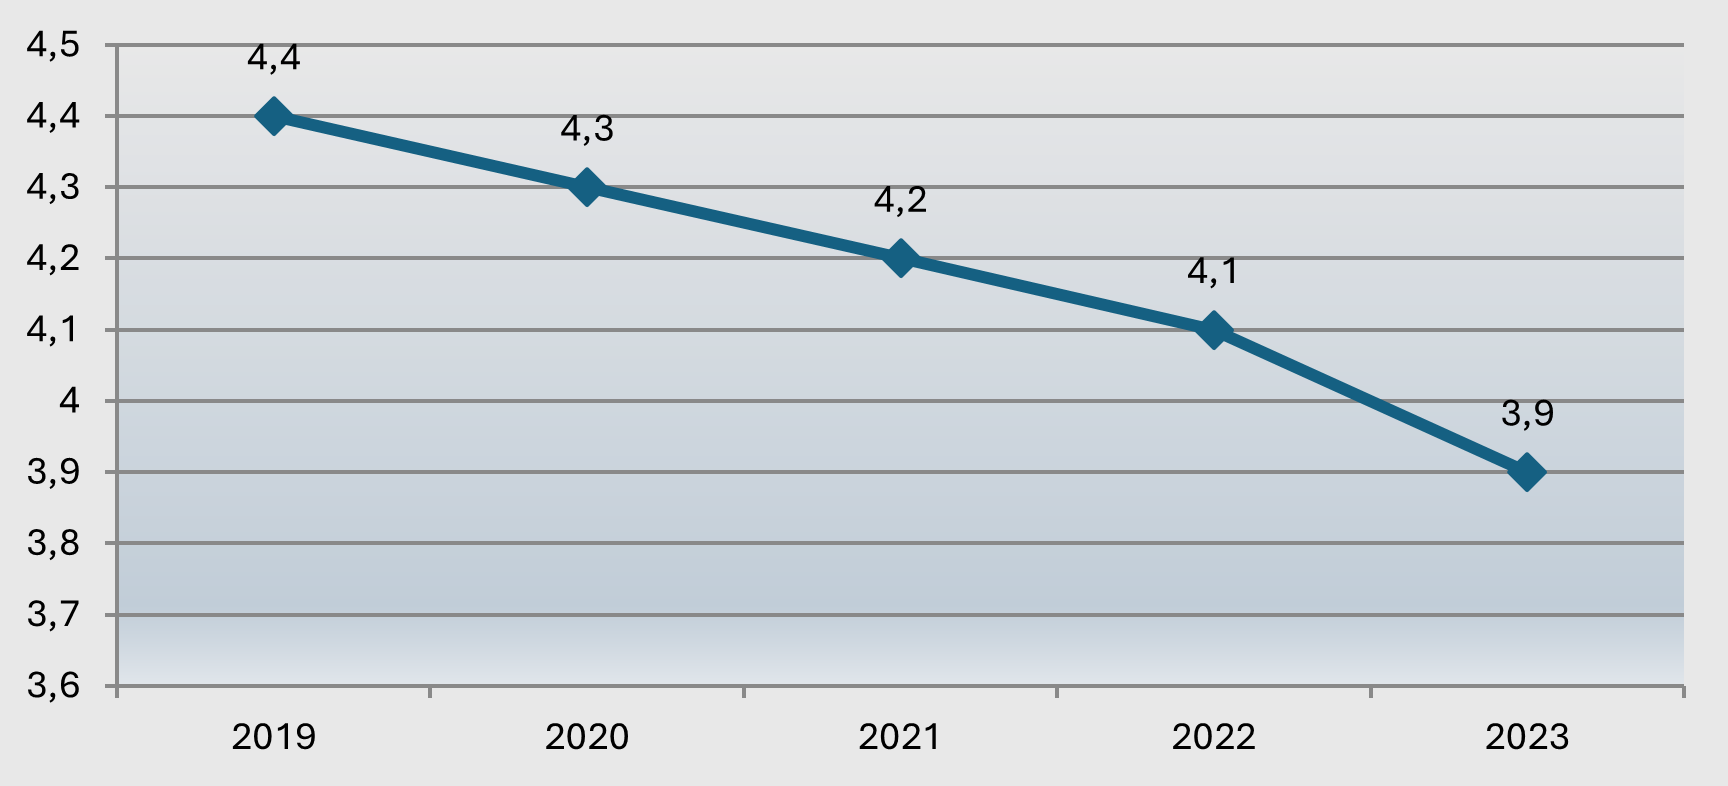
\includegraphics[width=0.8\textwidth]{media/ekon4/image3}
	\caption*{Рис.1 - Доля ВВП сельскохозяйственной отрасли}
	\caption*{\normalfont\emph{Примечание -- составлено авторами на основании {[}5{]}}}
\end{figure}

\begin{multicols}{2}
При этом валовой выпуск продукции сельского хозяйства за тот же период
снизился до 7,6 трлн тенге, прервав восходящую динамику, зафиксированную
в 2020--2022 годах (таблица 1).

Анализ динамики валового выпуска сельскохозяйственной продукции за
2018--2023 годы показывает, что с 2018 по 2022 год объемы выросли на 87
\% - с 4,47 трлн. до 8,37 трлн. тенге. Главным источником этого роста
стало растениеводство, где объёмы производства за указанный период более
чем удвоились. Однако в 2023 году общий выпуск сократился на 9,5 \%, из
них по растениеводству - на 1,26 трлн. тенге. На этом фоне наблюдается
частичное восстановление животноводства, что указывает на смещение
акцентов и внутренние дисбалансы в отраслевой структуре.
\end{multicols}

\tcap{Таблица 1 - Валовой выпуск продукции сельского хозяйства Казахстана (в млн тенге)}
\begin{longtblr}[
  label = none,
  entry = none,
]{
  width = \linewidth,
  colspec = {Q[63]Q[173]Q[183]Q[185]Q[121]Q[208]},
  cells = {c},
  cell{8}{1} = {c=6}{},
  hlines,
  vlines,
}
Год & Валовой
			выпуск & Растениеводство & Животноводство & С/х
			услуги & Темп
			прироста (\%)\\
2018 & 4
			474 088 & 2
			411 487 & 2
			050 456 & 12
			145 & -\\
2019 & 5
			151 163 & 2
			817 661 & 2
			319 497 & 14
			006 & 15,1\\
2020 & 6
			334 669 & 3
			687 310 & 2
			637 461 & 9
			898 & 23\\
2021 & 7
			515 433 & 4
			387 237 & 3
			116 974 & 11
			223 & 18,6\\
2022 & 8
			367 690 & 5
			808 260 & 2
			545 267 & 14
			162 & 11,3\\
2023 & 7
			576 534 & 4
			552 417 & 3
			012 510 & 11
			607 & –9,5\\
Примечание			– составлено авторами на основании			[5] &  &  &  &  & 
\end{longtblr}

\begin{multicols}{2}
При этом возвращение к прежним темпам роста без изменения самой модели
организации агропроизводства выглядит маловероятным, что подтверждает
необходимость глубоких преобразований, в том числе через объединение
производителей в партнёрские и кооперативные структуры.

Сельскохозяйственные формирования являются не только основными
производителями аграрной продукции, но и основой для создания устойчивых
предпринимательских сетей. Именно на уровне этих хозяйств сосредоточены
ключевые ресурсы: инициативность, труд, производственные мощности - все
то, что может стать фундаментом для горизонтальных и вертикальных связей
в агросекторе. По состоянию на 2023 год в Казахстане насчитывается более
330 тысяч таких формирований, причём подавляющее большинство из них ---
это малые хозяйства. Такая структура сама по себе несет ряд ограничений.
Небольшие предприятия, как правило, не имеют достаточных ресурсов для
модернизации, выхода на внешние рынки, участия в переработке или
создания собственной логистики.

Распределение сельскохозяйственные формирования по регионам с учётом их
специализации (растениеводство и животноводство) позволит точнее понять
географическую структуру аграрного производства в Казахстане. В таблице
2 приведены данные о численности хозяйствующих субъектов по областям, с
указанием преобладающего направления деятельности, что позволит увидеть
региональные различия и оценить, где есть потенциал для создания
предпринимательских сетей, соответствующих специфике местного сельского
хозяйства.

Проведенный анализ показывает, что распределение сельхозформирований по
регионам страны довольно неравномерный - как по количеству, так и по
специализации. Больше всего хозяйств сосредоточено в Туркестанской -
32~910 единиц, Костанайской и Акмолинской 25~752 единиц и 23~932 единиц
соответственно. Это во многом объясняется развитой системой
землепользования и исторически сложившейся аграрной направленностью этих
территорий.

Костанайская, Туркестанская, Северо-Казахстанская и Акмолинская области
лидируют по специализации растениеводство и формируют основу зернового
пояса Казахстана. В то же время животноводческие хозяйства занимают
доминирующее положение в Жамбылской, Абайской и Алматинской областях -
здесь на выбор специализации повлияли природные условия и наличие
пастбищ.
\end{multicols}

\tcap{Таблица 2 -- Сельскохозяйственные формирования по регионам и видам деятельности, 2023 г.}
\begin{longtblr}[
  label = none,
  entry = none,
]{
  row{1} = {c},
  row{23} = {c},
  cell{2}{2} = {c},
  cell{2}{3} = {c},
  cell{2}{4} = {c},
  cell{3}{2} = {c},
  cell{3}{3} = {c},
  cell{3}{4} = {c},
  cell{4}{2} = {c},
  cell{4}{3} = {c},
  cell{4}{4} = {c},
  cell{5}{2} = {c},
  cell{5}{3} = {c},
  cell{5}{4} = {c},
  cell{6}{2} = {c},
  cell{6}{3} = {c},
  cell{6}{4} = {c},
  cell{7}{2} = {c},
  cell{7}{3} = {c},
  cell{7}{4} = {c},
  cell{8}{2} = {c},
  cell{8}{3} = {c},
  cell{8}{4} = {c},
  cell{9}{2} = {c},
  cell{9}{3} = {c},
  cell{9}{4} = {c},
  cell{10}{2} = {c},
  cell{10}{3} = {c},
  cell{10}{4} = {c},
  cell{11}{2} = {c},
  cell{11}{3} = {c},
  cell{11}{4} = {c},
  cell{12}{2} = {c},
  cell{12}{3} = {c},
  cell{12}{4} = {c},
  cell{13}{2} = {c},
  cell{13}{3} = {c},
  cell{13}{4} = {c},
  cell{14}{2} = {c},
  cell{14}{3} = {c},
  cell{14}{4} = {c},
  cell{15}{2} = {c},
  cell{15}{3} = {c},
  cell{15}{4} = {c},
  cell{16}{2} = {c},
  cell{16}{3} = {c},
  cell{16}{4} = {c},
  cell{17}{2} = {c},
  cell{17}{3} = {c},
  cell{17}{4} = {c},
  cell{18}{2} = {c},
  cell{18}{3} = {c},
  cell{18}{4} = {c},
  cell{19}{2} = {c},
  cell{19}{3} = {c},
  cell{19}{4} = {c},
  cell{20}{2} = {c},
  cell{20}{3} = {c},
  cell{20}{4} = {c},
  cell{21}{2} = {c},
  cell{21}{3} = {c},
  cell{21}{4} = {c},
  cell{22}{2} = {c},
  cell{22}{3} = {c},
  cell{22}{4} = {c},
  cell{23}{1} = {c=4}{0.934\linewidth},
  hlines,
  vlines,
}
Регион & Всего формирований & Растениеводство & Животноводство\\
Абай & 7 244 & 2 056 & 5 188\\
Акмолинская & 23 932 & 14 830 & 9 102\\
Актюбинская & 7 572 & 5 013 & 2 559\\
Алматинская & 22 642 & 13 058 & 9 584\\
Атырауская & 3 483 & 1 219 & 2 264\\
Западно-Казахстанская & 14 206 & 7 874 & 6 332\\
Жамбылская & 21 147 & 9 012 & 12 135\\
Жетысу & 11 435 & 5 525 & 5 910\\
Карагандинская & 10 466 & 4 910 & 5 556\\
Костанайская & 25 752 & 19 476 & 6 286\\
Кызылординская & 11 017 & 8 013 & 3 004\\
Мангистауская & 1 396 & 999 & 397\\
Павлодарская & 8 366 & 5 686 & 2 680\\
Северо-Казахстанская & 18 433 & 15 528 & 2 905\\
Туркестанская & 32 910 & 27 167 & 5 743\\
Ұлытау & 2 820 & 1 981 & 839\\
Восточно-Казахстанская & 14 492 & 9 921 & 4 571\\
г. Астана & 110 & 49 & 61\\
г. Алматы & 86 & 23 & 63\\
г. Шымкент & 178 & 58 & 120\\
Итого по РК & 330 512 & 216 398 & 114 114\\
Примечание –				составлено авторами на основании [5] &  &  & 
\end{longtblr}

\begin{multicols}{2}
В крупных городах --- Астане, Алматы и Шымкенте - сельхозформирований
немного, что конечно же связано с ограниченностью сельскохозяйственных
земель и спецификой городской экономики.

Таким образом, сложившаяся региональная специализация аграрного
производства позволяет выстраивать предпринимательские сети с учетом
территориальной привязки и преобладающих направлений - зерноводство,
овощеводство, молочное и мясное животноводство и т.д. При этом явный
перекос в сторону растениеводства (на его долю приходится более 65 \%
всех формирований) указывает на необходимость выравнивания
производственной структуры, особенно в части развития цепочек
переработки и сбыта животноводческой продукции в южных и горных регионах
страны.

Несмотря на большое количество сельхозпроизводителей, переработка
продукции в стране по-прежнему сосредоточена в относительно небольшом
числе предприятий. По данным на 2023 год, в Республике Казахстан
зарегистрировано около 3 273 юридических лиц, занимающихся производством
продуктов питания --- это менее 1 \% от общего числа
сельхозформирований. Такая диспропорция указывает на сохраняющийся
разрыв между первичным производством и переработкой (рисунок 2).
\end{multicols}

\begin{figure}[H]
	\centering
	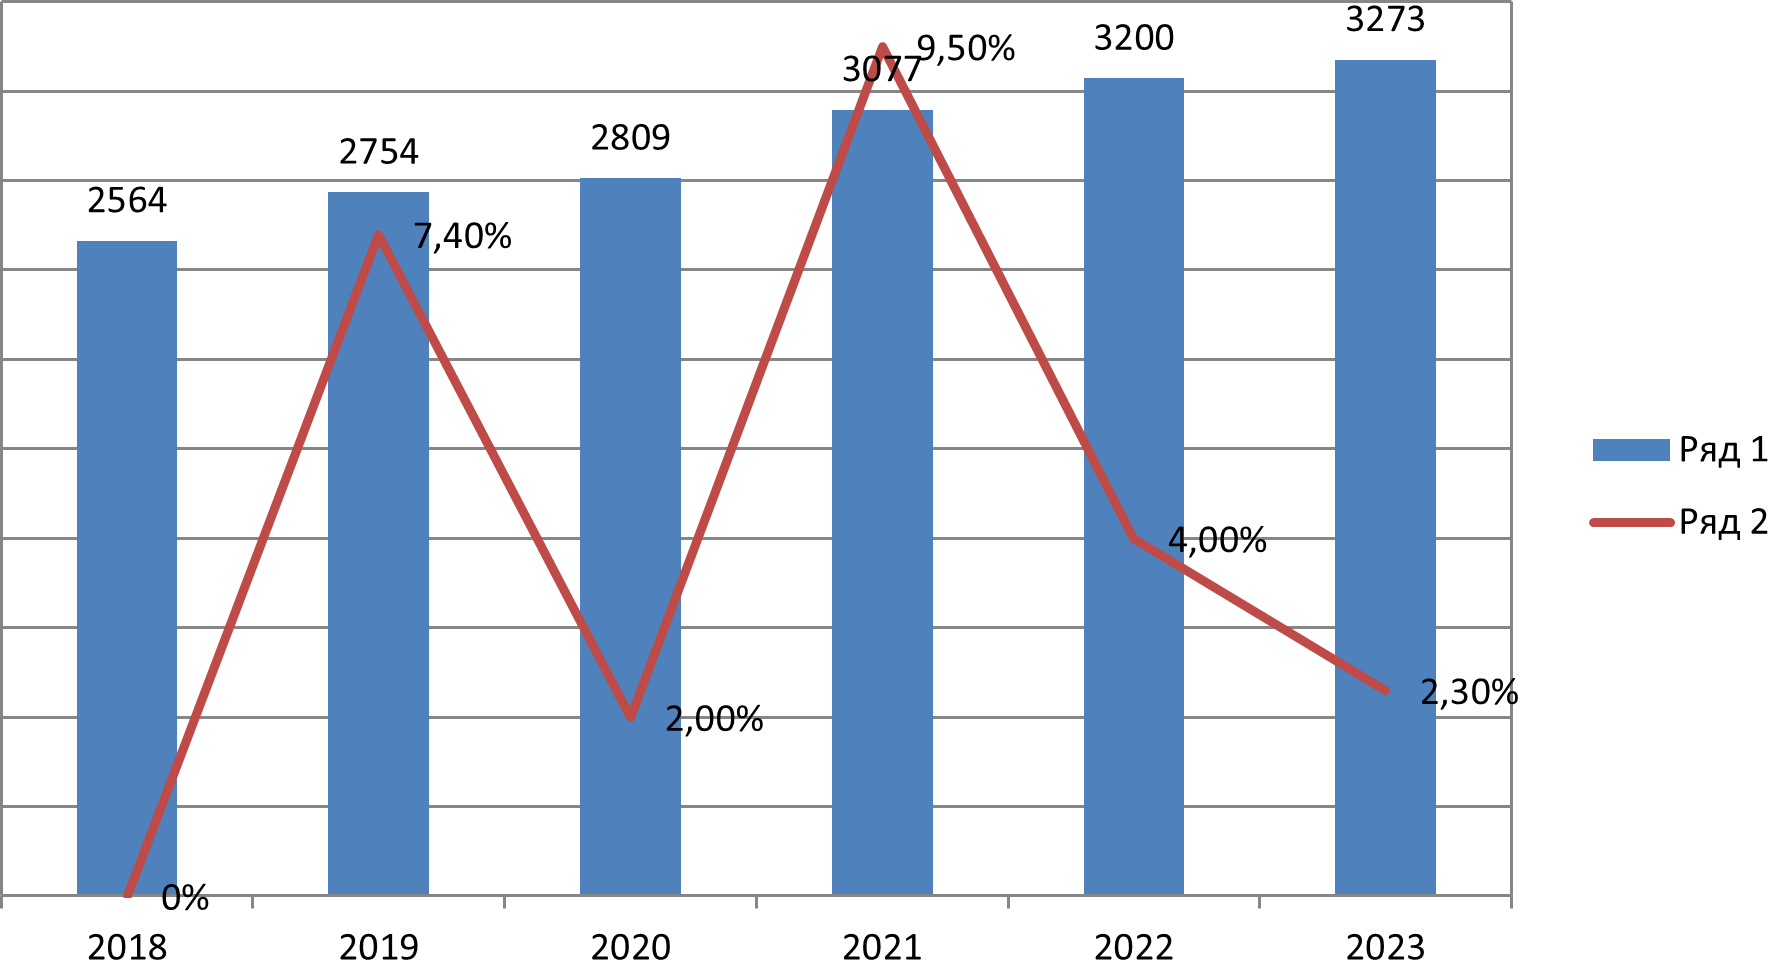
\includegraphics[width=0.8\textwidth]{media/ekon4/image4}
	\caption*{Рис.2 - Динамика и прирост количества предприятий пищевой промышленности в РК}
	\caption*{\normalfont\emph{Примечание -- составлено авторами на основании {[}8{]}}}
\end{figure}

\begin{multicols}{2}
Хотя общее количество перерабатывающих предприятий постепенно
увеличивается, с 2021 года темпы этого роста замедлились до 2-4 \% в
год, что говорит о том, что вход в отрасль остаётся затруднённым из-за
высокой капиталоёмкости, слабой логистической базы и недостаточной
кооперации с сельхозпроизводителями. Без создания условий для вовлечения
малых хозяйств в переработку через предпринимательские сети, потенциал
развития пищевой промышленности будет использоваться не в полной мере.

Наибольшее число пищевых производств сосредоточено в Алматинской области
- здесь развиты молочные, мясные и мукомольные направления.
Зернопереработка и хлебобулочное производство наиболее активно
развиваются в Костанайской и Карагандинской областях. В Туркестанской и
Жамбылской областях преобладает переработка овощей, фруктов и
безалкогольных напитков. Город Алматы остаётся важным центром выпуска
упакованных продуктов питания и полуфабрикатов.

В то же время в таких регионах, как Мангистауская, Атырауская и Ұлытау,
перерабатывающая отрасль развита слабо, что обусловлено как
географическими условиями, так и нехваткой соответствующей
инфраструктуры.

Инвестиционная активность - один из ключевых факторов, от которого
напрямую зависит возможность формирования и устойчивого развития
агропредпринимательских сетей. Без системного увеличения вложений в
сельское производство, переработку, логистику и объекты хранения
наладить прочные связи между хозяйствами и отраслями практически не
возможно. Поэтому необходимо смысл проанализировать, как менялась
динамика инвестиций в основной капитал в сельском хозяйстве и смежных
сферах - это может служить косвенным показателем того, насколько отрасль
готова к изменениям и к переходу к сетевым форматам взаимодействия.

Несмотря на рост в абсолютных значениях - с 12,6 трлн. тенге в 2019 году
до 17,6 трлн. тенге в 2023 году - доля аграрного сектора в общем объёме
инвестиций после 2021 года снижается - с 5,83 \% до 5,12 \% (рисунок 3).
Это может свидетельствовать о снижении привлекательности отрасли для
инвесторов на фоне сохраняющихся барьеров.
\end{multicols}

\begin{figure}[H]
	\centering
	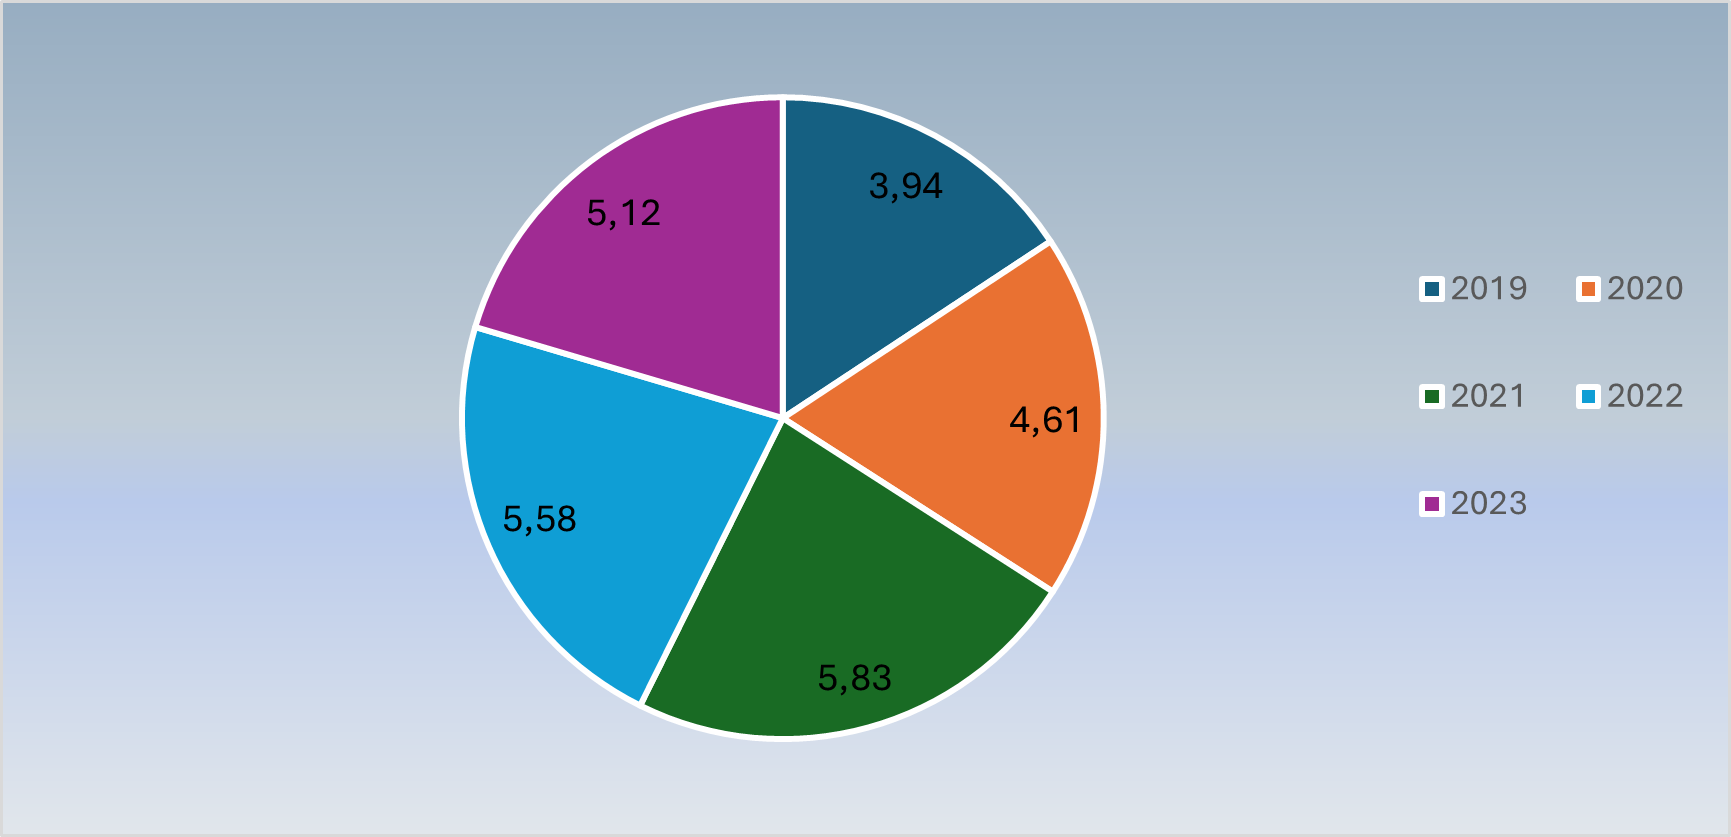
\includegraphics[width=0.8\textwidth]{media/ekon4/image5}
	\caption*{Рис.3 - Инвестиции в основной капитал агросектора в общем объёме инвестиций (2019--2023 гг.)}
	\caption*{\normalfont\emph{Примечание -- составлено авторами на основании {[}7{]}}}
\end{figure}

\begin{multicols}{2}
Анализ инвестиций показал, что особо остро нехватка инвестиций ощущается
в сегменте переработки. Обрабатывающая промышленность, особенно ее
пищевое звено, играет ключевую роль в агропромышленной цепочке, ведь
именно здесь создается добавленная стоимость, а сельхозпродукция
превращается в готовый продукт для рынка. Однако данные показывают, что
на производство продуктов питания стабильно направляется менее 10 \% от
общего объёма инвестиций в обрабатывающую отрасль. Это говорит о том,
что масштаб модернизации остается ограниченным и основной причиной
является слабая интеграция с производственными организациями и нехватка
устойчивых связей между фермерами и переработчиками.
\end{multicols}

\tcap{Таблица 3 - Инвестиции в обрабатывающую промышленность по видам деятельности (2019--2023 гг.), млн тенге}
\begin{longtblr}[
  label = none,
  entry = none,
]{
  width = \linewidth,
  colspec = {Q[50]Q[240]Q[137]Q[75]Q[137]Q[77]Q[77]Q[135]},
  cells = {c},
  cell{7}{1} = {c=8}{0.927\linewidth},
  hlines,
  vlines,
}
\textbf{Год} & \textbf{Обрабатывающая				промышленность} & \textbf{Продукты питания} & \textbf{Напи\-тки} & \textbf{Табачные изделия} & \textbf{Тек\-стиль} & \textbf{Одеж\-да} & \textbf{Кожаные изделия}\\
2019 & 1 017 089 & 90 154 & 24 361 & 8 835 & 7 684 & 434 & 1 134\\
2020 & 1 077 819 & 109 055 & 21 908 & 10 104 & 2 905 & 1 218 & 1 229\\
2021 & 1 541 742 & 118 315 & 32 699 & 7 655 & 4 334 & 1 258 & 282\\
2022 & 1 586 872 & 140 439 & 26 234 & 9 578 & 5 075 & 1 325 & 623\\
2023 & 1 633 025 & 156 874 & 45 258 & 23 873 & 10 965 & 2 870 & {~\\~}\\
Примечание –				составлено авторами на основании [7] &  &  &  &  &  &  & 
\end{longtblr}

\begin{multicols}{2}
Даже при наращивании финансирования ввод новых перерабатывающих
мощностей остаётся точечным и ограниченным. В 2023 году, согласно данным
по вводу объектов, новые производственные мощности появились лишь в
отдельных секторах, преимущественно в форме малых предприятий (таблица
4)
\end{multicols}

\tcap{Таблица 4 - Ввод в эксплуатацию перерабатывающих объектов в 2023 году}
\begin{longtblr}[
  label = none,
  entry = none,
]{
  width = \linewidth,
  colspec = {Q[312]Q[125]Q[217]Q[283]},
  cells = {c},
  cell{7}{1} = {c=4}{0.937\linewidth},
  hlines,
  vlines,
}
\textbf{Вид			объекта} & \textbf{Кол-во			объектов} & \textbf{Совокупная			мощность (тонн/год)} & \textbf{Основные			регионы}\\
Предприятия
			по производству мяса и мясопродуктов & 4 & 8
			152 & Акмолинская,
			Алматинская, Жамбылская, Ұлытау\\
Рыбоводные
			хозяйства (товарная рыба) & 3 & 1
			220 & Алматинская,
			Жамбылская, Костанайская\\
Предприятия
			по переработке и консервированию рыбы & 2 & 213 & Туркестанская,
			ВКО\\
Производство
			растительных и животных масел & 1 & 6
			336 & Костанайская\\
Производство
			молочной продукции & 3 & 885 & Жамбылская,
			Кызылординская, Туркестанская\\
Примечание			– составлено авторами на основании			[8] &  &  & 
\end{longtblr}

\begin{multicols}{2}
Необходимо отметить, объемы производственных мощностей остаются
сравнительно низкими, особенно с учётом масштабов сельскохозяйственного
производства в стране. Это указывает на структурный разрыв между
первичным производством и переработкой, который мог бы быть преодолен за
счет расширения партнёрских предпринимательских сетей - особенно
кооперативного типа, с возможностью коллективного инвестирования и
совместного использования инфраструктуры.

Необходимо отметить, что объемы производственных мощностей остаются
относительно низкими, особенно если учитывать масштабы отечественного
сельскохозяйственного производства, что говорит о сохраняющемся разрыве
между первичным производством и переработкой. Данную проблему возможно
преодолеть за счет развития партнерских предпринимательских сетей, в
первую очередь через кооперативные формы, где хозяйства могли бы
вкладываться вместе и использовать инфраструктуру на правах партнерства.

Однако формирование устойчивых предпринимательских связей в
агропромышленном комплексе требует не только инвестиций, но и
научно-технической базу. Выстраивание эффективной системы координации и
поддержки в аграрной сфере невозможно без системной поддержки научных
исследований и технологической модернизации. В данном контексте,
особенно важно состояние и структура внутренних затрат на
научно-исследовательские и опытно-конструкторские работы. В 2023 году
они составили 12,2 млрд. тенге, что составляет лишь 5,6\% от общих
затрат на НИОКР в стране. Из этой суммы 71,7\% было направлено на оплату
труда исследователей, тогда как на приобретение оборудования --- менее
1\% (рисунок 4).
\end{multicols}

\begin{figure}[H]
	\centering
	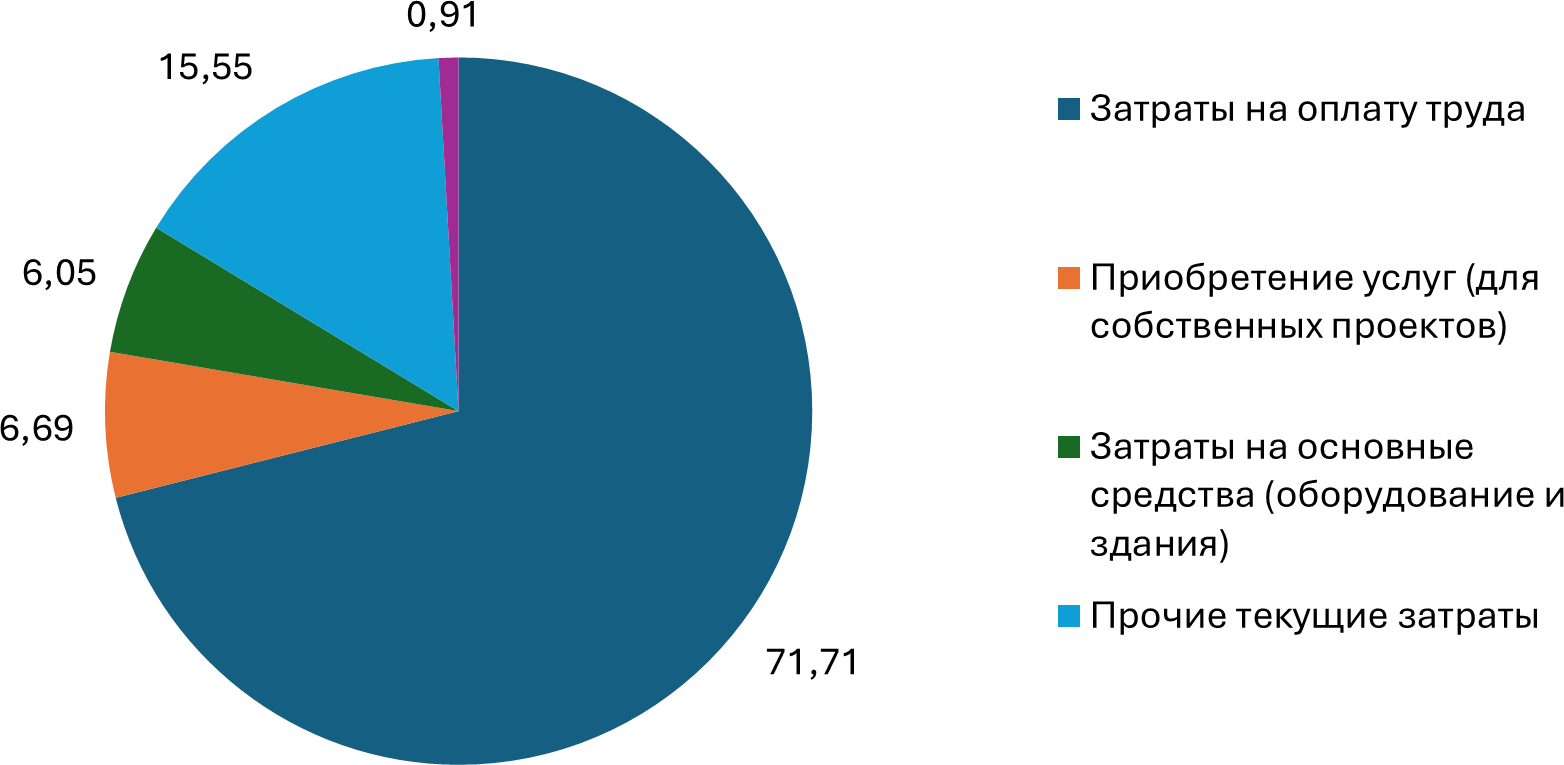
\includegraphics[width=0.7\textwidth]{media/ekon4/image6}
	\caption*{Рис.4 - Структура внутренних затрат на НИОКР по сельскохозяйственным наукам в 2023 году, тыс. тг}
	\caption*{\normalfont\emph{Примечание -- составлено авторами на основании {[}8{]}}}
\end{figure}

\begin{multicols}{2}
Несмотря на то, что сельское хозяйство считается важным для
продовольствия и занятости, инновационная активность остается крайне
низкой. По последним данным, только около 10\% хозяйств пробовали
внедрять те или иные инновационные методы и технологии в производстве, а
доля такой продукции в общем выпуске - меньше 1\%. И как показывает
анализ, большая часть вложений в инновации направлены на улучшение
бизнес-процессов (логистика, управление), а на новые технологии и товары
- меньше 4 млрд тенге, и это еще раз подчеркивает, что на слабую
ориентацию технологического обновления в аграрной сфере и отсутствие
стимулов к внедрению агротехнологий. Все это сдерживает развитие
партнерских предпринимательских сетей, в том числе тех, что могли бы
строиться вокруг совместных инновационных решений.

{\bfseries Выводы.} Результаты проведенного анализа позволяют авторам
сделать вывод о наличии системных ограничений, тормозящих устойчивое
развитие агропромышленного комплекса Казахстана. Можно отметить, что
несмотря на то, что происходит рост производства и численности
сельхозформирований, при этом сохраняется фрагментарность отрасли,
присутствует слабая интеграция между производством, переработкой и
сбытом, а также фиксируется недостаточная вовлеченность малых и средних
хозяйств в инфраструктурные и инновационные процессы.

Обнаруженная исследователями несбалансированность в отраслевой структуре
говорит о перекосе в сторону растениеводства при слабой развитости
цепочек переработки животноводческой продукции. С точки зрения
формирования устойчивых межхозяйственных и межотраслевых связей
инвестиционная активность в аграрном секторе остается недостаточной, что
особенно касается сегмента пищевой переработки, доля которой в общем
объеме инвестиций в обрабатывающую промышленность низкая.

Инновационный потенциал сектора также реализуется слабо. Большая часть
затрат, направленных на инновации, внедряется на улучшение
бизнес-процессов, тогда как создание новых агротехнологий и
инновационных продуктов эпизодические. Отсутствие каналов трансфера
знаний, слабая научная база и низкий уровень цифровизации в большинстве
регионов усиливают институциональную уязвимость сектора.

В этих условиях формирование партнерских предпринимательских сетей
представляет собой перспективный, но пока недостаточно реализованный
механизм преодоления структурной разрозненности. Такие сети могут стать
инструментом координации усилий между производителями, переработчиками,
логистическими, научными и финансовыми структурами, а также основой для
повышения устойчивости и конкурентоспособности агропромышленного
комплекса в целом.
\end{multicols}

\begin{center}
{\bfseries Литература}
\end{center}

\begin{references}
1. Концепция развития агропромышленного комплекса Республики Казахстан
на 2021--2030 годы, утверждённая постановлением Правительства РК от 28
декабря 2021 года № 960. URL:\\
\href{https://adilet.zan.kz/rus/docs/P2100000960}{https://adilet.zan.kz} .- Дата обращения:
05.06.2025

2. Закон Республики Казахстан «О сельскохозяйственных кооперативах» от
29 октября 2015 года № 372-V ЗРК. URL:
\href{https://adilet.zan.kz/rus/docs/Z1500000372}{https://adilet.zan.kz} - Дата обращения:
05.06.2025

3. Обзор развития сельского хозяйства в Казахстане (FAO, 2022). URL:
\href{https://openknowledge.fao.org/bitstream/handle/20.500.14283/cc2651ru.pdf}{https://openknowledge.fao.org}
Дата обращения: 05.06.2025.

4. Сельское хозяйство Республики Казахстан (1 том, 2 том):
Статистический сборник. -- Бюро национальной статистики РК. - 2023.
URL: \href{https://stat.gov.kz/ru/publication/collections/?year=2023&name=17199&period=year}{https://stat.gov.kz}
-Дата обращения: 05.06.2025

5. О деятельности сельскохозяйственных кооперативов в Республике
Казахстан за 2023 год. URL:
\href{https://stat.gov.kz/api/iblock/element/182382/file/ru/}{https://stat.gov.kz} -Дата
обращения: 05.06.2025.

6. Инновационная активность организаций по видам экономической
деятельности. Бюро национальной статистики РК. - 2023. URL:
\href{https://stat.gov.kz/ru/industries/business-statistics/stat-inno-build/publications}{https://stat.gov.kz}
- Дата обращения: 05.06.2025

7. Инвестиционная и строительная деятельность в Республике Казахстан:
статистический сборник. - Астана: Бюро национальной статистики Агентства
по стратегическому планированию и реформам Республики Казахстан. - 2023.
URL:
\href{https://stat.gov.kz/ru/publication/collections/?year=2023&name=16821&period=year}{https://stat.gov.kz}
- Дата обращения: 05.06.2025

8. Показатели индустриально-инновационного развития Республики
Казахстан: статистический сборник. - Астана: Бюро национальной
статистики Агентства по стратегическому планированию и реформам
Республики Казахстан. - 2022.
URL: \href{https://stat.gov.kz/ru/publication/collections/?year=2022&name=16147&period}{https://stat.gov.kz}
- Дата обращения: 05.06.2025

9. Керимова У. К., Касенбаев Г. С. Ключевые проблемы развития
агропромышленного комплекса в Казахстане и пути их решения // Вестник
университета «Туран». -- 2021. -- №1(101). - С.85-92. DOI
10.46914/1562-2959-2021-1-4-85-92

10. Женсхан Д., Мусаева М. А., Сабырова М. Е., Қазкен Г. Д.
Қазақстандағы ауыл шаруашылығы кооперативтері: даму жағдайы, мәселелері
және дамыту тетіктері // Тұран университетінің хабаршысы. - 2025.- №
1(105).- С.168-180. DOI 10.46914/1562-2959-2025-1-1-168-180

11. Аймурзина Б. Т., Каменова М. Ж., Ержанова С. К., Спанова Б. К.
Развитие сельскохозяйственной кооперации в Казахстане // Вестник
Казахского университета экономики, финансов и международной торговли
(КУЭФ). - 2022. - № 2. - С.4251. DOI 10.52260/2304-7216.2022.3(48).1

12. Абдыкалиева Ж.Ш., Казиева А.Н., Маевский Д.П. Сельскохозяйственная
кооперация\\
в Казахстане: состояние и потенциальные возможности// Проблемы
агрорынка. - 2021. - № 2. - С.16-29. DOI 10.46666/2021-2.2708-9991.21

13. Митин Д. А. Сущность кооперации и её роль в развитии аграрного
сектора экономики //Экономика и предпринимательство. - 2018.- № 12(89).-
С.1013--1016.

14. Ахметов В. Я. Роль кооперации субъектов агробизнеса в повышении
конкурентоспособности сельской экономики (на примере районов Зауралья
Республики Башкортостан) // Российское предпринимательство. - 2015.- Т.
16 (10). - С.1505-1516. DOI 10.18334/rp.16.10.258

15. Kar S., Das S., Kar B. Networking Behaviour of Agri-entrepreneurs
and Systematic Challenges. // SEDME (Small Enterprises Development,
Management \& Extension Journal). -- 2024. - Vol.51(1). - P.323--342.
DOI 10.1177/09708464241278463

16. Karami E., Keshavarz M. Collaborative Networking among Agricultural
Production Cooperatives: Mechanisms and Development. Heliyon.- 2020. -
6(4), e03893. DOI
\href{https://doi.org/10.1016/j.heliyon.2020.e03893}{10.1016/j.heliyon.2020.e03893}.

17. Klerkx L., Aarts N., Leeuwis, C. (2010). Adaptive management in
agricultural innovation systems: The interactions between innovation
networks and their environment. Agricultural Systems. - 2010. - Vol.
103(6). - P.390 - 400. DOI 10.1016/j.agsy.2010.03.012.
\end{references}

\begin{center}
{\bfseries References}
\end{center}

\begin{references}
1. Koncepcija razvitija agropromyshlennogo kompleksa Respubliki Kazahstan
na 2021--2030 gody, utver\-zhdjonnaja postanovleniem
Pravitel' stva RK ot 28 dekabrja 2021 goda № 960.
URL: \href{https://adilet.zan.kz/rus/docs/P2100000960}{https://adilet.zan.kz} - Data obrashhenija:
05.06.2025. {[}in Russian{]}

2. Zakon Respubliki Kazahstan «O sel' skohozjajstvennyh
kooperativah» ot 29 oktjabrja 2015 goda № 372-V ZRK. URL:
\href{https://adilet.zan.kz/rus/docs/Z1500000372}{https://adilet.zan.kz} - Data obrashhenija:
05.06.2025. .{[}in Russian{]}

3. Obzor razvitija sel' skogo hozjajstva v Kazahstane
(FAO, 2022). URL:
\href{https://openknowledge.fao.org/bitstream/handle/20.500.14283/cc2651ru.pdf}{https://openknowledge.fao.org}
- Data obrashhenija: 05.06.2025. .{[}in Russian{]}

4. Sel' skoe hozjajstvo Respubliki Kazahstan (1 tom, 2
tom): Statisticheskij sbornik. -- Bjuro nacional' noj
statistiki RK. - 2023.
URL: \href{https://stat.gov.kz/ru/publication/collections/?year=2023\&name=17199\&period=year}{https://stat.gov.kz}
-Data obrashhenija: 05.06.2025. .{[}in Russian{]}

5. O dejatel' nosti sel' skohozjajstvennyh
kooperativov v Respublike Kazahstan za 2023 god. URL:\\
\href{https://stat.gov.kz/api/iblock/element/182382/file/ru/}{https://stat.gov.kz} - Дata
obrashhenija 05.06.2025. {[}in Russian{]}

6. Innovacionnaja aktivnost'{} organizacij po vidam
jekonomicheskoj dejatel' nosti. Bjuro
nacional' noj statistiki RK. - 2023. URL:
\href{https://stat.gov.kz/ru/industries/business-statistics/stat-inno-build/publications}{https://stat.gov.kz}
- Data obrashhenija: 05.06.2025. {[}in Russian{]}

7. Investicionnaja i stroitel' naja
dejatel' nost'{} v Respublike Kazahstan:
statisticheskij sbornik. - Astana: Bjuro nacional' noj
statistiki Agentstva po strategicheskomu planirovaniju i reformam
Respubliki Kazah\-stan. - 2023. URL:
\href{https://stat.gov.kz/ru/publication/collections/?year=2023\&name=16821\&period=year}{https://stat.gov.kz}
- Data obrashhenija: 05.06.2025. {[}in Russian{]}

8. Pokazateli industrial' no-innovacionnogo razvitija
Respubliki Kazahstan: statisticheskij sbornik. - Astana: Bjuro
nacional' noj statistiki Agentstva po strategicheskomu
planirovaniju i reformam Respubliki Kazah\-stan. - 2022.
URL: \href{https://stat.gov.kz/ru/publication/collections/?year=2022\&name=16147\&period}{https://stat.gov.kz}
- Data obrashhenija: 05.06.2025. {[}in Russian{]}

9. Kerimova U. K., Kasenbaev G. S. Kljuchevye problemy razvitija
agropromyshlennogo kompleksa v Kazahstane i puti ih reshenija // Vestnik
universiteta «Turan». -- 2021. -- №1(101). - S.85-92. DOI\\
10.46914/1562-2959-2021-1-4-85-92. {[}in Russian{]}

10. Zhenshan D., Musaeva M. A., Sabyrova M. E., Қazken G. D.
Қazaқstandaғy auyl sharuashylyғy kooper\-ativterі: damu zhaғdajy,
mәselelerі zhәne damytu tetіkterі // Tұran universitetіnің habarshysy. -
2025. - № 1(105).- S.168-180. DOI
10.46914/1562-2959-2025-1-1-168-180.{[}in Kazakh{]}

11. Ajmurzina B. T., Kamenova M. Zh., Erzhanova S. K., Spanova B. K.
Razvitie sel' skohozjajstvennoj kooperacii v Kazahstane
// Vestnik Kazahskogo universiteta jekonomiki, finansov i mezhdunarodnoj
torg\-ovli (KUJeF). - 2022. - № 2. - S.4251. DOI
10.52260/2304-7216.2022.3(48).1. {[}in Russian{]}

12. Abdykalieva Zh.Sh., Kazieva A.N., Maevskij D.P.
Sel' skohozjajstvennaja kooperacija v
Kazahstane: sostojanie i potencial' nye vozmozhnosti//
Problemy agrorynka. - 2021. - № 2. - S.16-29. DOI\\
10.46666/2021-2.2708-9991.21. {[}in Russian{]}

13. Mitin D. A. Sushhnost'{} kooperacii i ejo
rol'{} v razvitii agrarnogo sektora jekonomiki
//Jekonomika i predprinimatel' stvo. - 2018.- № 12(89).-
S.1013--1016. {[}in Russian{]}

14. Ahmetov V. Ja. Rol'{} kooperacii sub\#ektov
agrobiznesa v povyshenii konkurentosposobnosti sel' skoj
jekonomiki (na primere rajonov Zaural' ja Respubliki
Bashkortostan) // Rossijskoe predprinimatel' stvo. -
2015. - T.16 (10). - S.1505-1516. DOI 10.18334/rp.16.10.258. {[}in
Russian{]}

15. Kar S., Das S., Kar B. Networking Behaviour of Agri-entrepreneurs
and Systematic Challenges. // SEDME (Small Enterprises Development,
Management \& Extension Journal). -- 2024. - Vol.51(1). - P.323--342.
DOI 10.1177/09708464241278463

16. Karami E., Keshavarz M. Collaborative Networking among Agricultural
Production Cooperatives: Mechanisms and Development. Heliyon.- 2020. -
6(4), e03893. DOI
\href{https://doi.org/10.1016/j.heliyon.2020.e03893}{10.1016/j.heliyon.2020.e03893}.

17. Klerkx L., Aarts N., Leeuwis, C. (2010). Adaptive management in
agricultural innovation systems: The interactions between innovation
networks and their environment. Agricultural Systems. - 2010. - Vol.
103(6). - P.390 - 400. DOI 10.1016/j.agsy.2010.03.012.
\end{references}

\begin{authorinfo}
\hspace{1em}\emph{{\bfseries Сведения об авторах}}

Юсупова С.А. - к.э.н., ст.преподаватель кафедры Экономика, Казахский
агротехнический исследовательский университет им. С. Сейфуллина, Астана,
Казахстан, e-mail: Abay.saltanat@bk.ru;

Толысбаева М.С. - асс. профессор кафедры Экономика, Казахский
агротехнический исследовательский университет имени С. Сейфуллина,
Астана, Казахстан, e-mail: tolysbayeva.m@mail.ru;

Касенова А. Ж. - к.э.н., асс.профессор кафедры Экономика, Казахский
агротехнический исследовательский университет им. С. Сейфуллина, Астана,
Казахстан, e-mail: Kasenova\_a@bk.ru;

Нарбаева Г.К. - старший преподаватель кафедры экономика, Казахский
агротехнический исследовательский университет им. С. Сейфуллина, Астана,
Казахстан, e-mail: narbaeva\_gulmira@mail.ru.

\hspace{1em}\emph{{\bfseries Information about the authors}}

Yussupova S. A. - PhD in Economics, Senior Lecturer Department of
Economics, Kazak Agrotechnical Research University named after S.
Seifullin, Astana, Kazakhstan, e-mail: Abay.saltanat@bk.ru;

Tolysbayeva M.S. - Associate Professor of the Department of Economics,
Kazak Agrotechnical Research University named after S. Seifullin,
Astana, Kazakhstan, e-mail: tolysbayeva.m@mail.ru;

Kasenova A. Zh.- Associate Professor of the Department of Economics, PhD
in Economics, Kazak Agrotechnical Research University named after S.
Seifullin, Astana, Kazakhstan, e-mail: Kasenova\_a@bk.ru;

Narbaeva G. K. - Senior Lecturer, Department of Economics, Kazakh
Agrotechnical Research University named after S. Seifullin, Astana,
Kazakhstan, e-mail: narbaeva\_gulmira@mail.ru.
\end{authorinfo}
